\documentclass[11pt]{article}
\usepackage[utf8]{inputenc}
\usepackage{amsmath}
\usepackage{amssymb}
\usepackage{graphicx}
\usepackage{hyperref}
\usepackage[parfill]{parskip}
\let\oldemptyset\emptyset
\let\emptyset\varnothing


\title{\textbf{Esssentials of Applied Data Analysis\\
				IPSA-USP Summer School 2017}\newline\\
				Discrete Random Variables}

\author{Leonardo Sangali Barone\\ \href{leonardo.barone@usp.br}{leonardo.barone@usp.br}}
\date{jan/17}

\begin{document}

\maketitle

\section*{Discrete Random Variables}

	We will start generating the discrete variables. We already know that variables are called \emph{random} variables because they can take values according to their probability.\\
	
	\subsection*{First example: \emph{sex} of fake citizens}
	
	Let's start with the \emph{sex} variable, which we will name $X$. Playing Fakeland's God, I am decided that the distribution of sex within fake citizens is:\\
	
\begin{tabular}{|c|c|c|}
\hline
	$i$ & $x_i$ & $P(X=x_i)$\\
	\cline{1-3}
	0 & "Male" & 0.40\\
	1 & "Female" & 0.60\\
\hline
\end{tabular}\\

$x_i$ are the values that the variable can assume (in this case, $x_1 = $ ``Male'' and $x_2 = $ ``Female''). Can you understantd this notation?\\

We can also write that the probability of our variable $X$ (\emph{sex}) beying equal $x_1$ (``Male'') is $P(X = x_1) = 0.4$. Again, can you understand this notation?\\

The table representes a probability distribution (or model) of a certain variable. It is no empirical, because it is the ``True'' distribution of sex in the Fakeland population.\\

We can also represent the distribution in a bar plot, as in Figure~\ref{f1}:

\begin{figure}[htp]
\centering
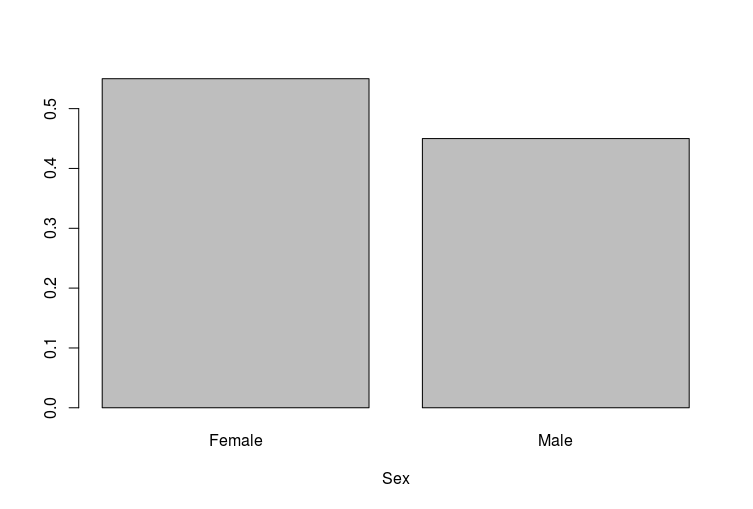
\includegraphics[scale=0.50]{sex_distribution.png}
\caption{Sex Distribution in Fakeland}
\label{f1}
\end{figure}

	\subsection*{Probability distribution \emph{vs} Sample distribution}

	Wait! But I have the fake dataset in my hands and, after counting it, I found out that there are 15 men and 15 women among the 30! How can we have 2 different distributions?\\

	While playing God, I draw from the probability distribution that generates all the data in the world of Fakeland. For example, when we roll a dice or toss a coin, we know the process that generate the data (and define the probabilities for each event) and that is why we are able to compute probabilities without actually rolling the dice or tossing the coin.\\
	
	However, when we are working with human beings, we rarely have the oportunity to get to know the process that generate the data (even when we collect census data). That is why we work with samples.\\
	
	What you have in your hands is a sample of Fakeland individuals. Randomness was responsable for picking 15 men and 15 women, even thought we were expecting 12 man and 18 women.\\

	We differentiate probability distribution from a sample distribution. We can build a sample distribiution from a frequency table (ocurrences of the variable in the sample!). More generally, we can say we build distribuitions from the realizations of the variable (e.g. number of seats in a Legislative, Moore and Siegel, ch 10, pp. 202-203).\\
	
	We can represent our sample distribution as follows:\\
	
\begin{tabular}{|c|c|c|}
\hline
	$i$ & $x_i$ & $f(x_i)$\\
	\cline{1-3}
	0 & "Male" & 0.50\\
	1 & "Female" & 0.50\\
\hline
\end{tabular}\\
	
	Where $f(x_i)$ means the \emph{relative frequency} of $x_i$ in our sample.//

	Take a moment to see if you can understand this very important difference.

	\subsection*{Why do we sample?}
	
	If the probability distribution is unknown, we can try to \textbf{estimate} it by taking the sample distribution. Let's look fot the other discrete variables in the fake dataset. All of the tables contain both the probability distribution that generated the sample and the sample distribution. For the sake of simplicity, we called all the variables as $X$, but you can use any other letter ($Y$ and $Z$ are also very common) or even subscripts (as in $X_1 ... X_n$).\\
	
	Educational Level:
	
\begin{tabular}{|c|c|c|c|}
\hline
	$i$ & $x_i$ & $P(X=x_i)$ & $f_i$\\
	\cline{1-4}
	1 & "No High School Degree" & 0.10 & 0.10\\
	2 & "High School Degree" & 0.40 & 0.47\\
	3 & "College Incomplete" & 0.20 & 0.2\\
	4 & "College Degree or more" & 0.30 & 0.23\\	
\hline
\end{tabular}\newline\\

Marriage Status (Married = Yes):

\begin{tabular}{|c|c|c|c|}
\hline
	$i$ & $x_i$ & $P(X=x_i)$ & $f_i$\\
	\cline{1-4}
	0 & "Yes" & 0.50 & 0.53\\
	1 & "No" & 0.50 & 0.47\\
\hline
\end{tabular}\newline\\

Number of Children:

\begin{tabular}{|c|c|c|c|}
\hline
	$i$ & $x_i$ & $P(X=x_i)$ & $f_i$\\
	\cline{1-4}
	1 & "0" & 0.50 & 0.73\\
	2 & "1" & 0.25 & 0.13\\
	3 & "2" & 0.20 & 0.07\\
	4 & "3 or more" & 0.05 & 0.07\\	
\hline
\end{tabular}\newline\\

Party affiliation:

\begin{tabular}{|c|c|c|c|}
\hline
	$i$ & $x_i$ & $P(X=x_i)$ & $f_i$\\
	\cline{1-4}
	1 & "Conservative Party" & 0.20 & 0.20\\
	2 & "Socialist Party" & 0.20 & 0.30\\
	3 & "Independent" & 0.60 & 0.50\\
\hline
\end{tabular}\newline\\

Vote History (observe that this is the only integer variable in our dataset and there is no need to associate an $i$ with each $x_i$):

	\begin{tabular}{|c|c|}
\hline
	$i = x_i$ & $P(X=x_i)$\\
	\cline{1-2}
	0 & 0.30\\
	1 & 0.10\\
	2 & 0.10\\
	3 & 0.20\\
	4 & 0.30\\
\hline
\end{tabular}


\subsection*{Exercise}

Build the sample distribution for the other discrete variables in the dataset using the relative frequencies.

\section*{Discrete Random Variables - Dices and Coins}

	Let's take a look at classical dices and coins examples of discrete random variables.

	\subsection*{Dices and coins - Examples}
		
	A) Let's call $X$ the variable that indicates the result we obtain when we roll a 6-side dice. This variable can assume 6 different values, \{1,2,3,4,5,6\}, and all of them have the same probability, $P(X=x_i) = 1/6$.\\
	
	\begin{tabular}{|c|c|}
\hline
	$x_i$ & $P(X=x_i)$\\
	\cline{1-2}
	1 & 1/6\\
	2 & 1/6\\
	3 & 1/6\\
	4 & 1/6\\
	5 & 1/6\\
	6 & 1/6\\

\hline
\end{tabular}\newline\\

Note: The realization of a random variable is a particular value that it takes and we usually represent it with a small letter (e.g. $x_i$ is a realization of $X$).\\

	B) Let's call $Y$ the variable that indicates the result we obtain when we roll a pair of dice and sum the results. What is the distribution of $Y$?\\
	
	\begin{tabular}{|c|c|c|c|}
\hline
	$y_i$ & $P(Y=y_i)$ & $y_i$ & $P(Y=y_i)$\\
	\cline{1-4}
	1 & 0 & 7 & 6/36\\
	2 & 1/36 & 8 & 5/36\\
	3 & 2/36 & 9 & 4/36\\
	4 & 3/36 & 10 & 3/36\\
	5 & 4/36 & 11 & 2/36\\
	6 & 5/36 & 12 & 1/36\\
\hline
\end{tabular}\newline\\

	C) Let's call $X$ the variable that indicates the number of heads we obtain when we toss a coin 5 times. This variable can assume 6 different values: \{0,1,2,3,4,5\}.\\
	
	\begin{tabular}{|c|c|}
\hline
	$x_i$ & $P(X=x_i)$\\
	\cline{1-2}
	0 & $(0.5)^5$\\
	1 & $(0.5)^1$\\
	2 & $(0.5)^2$\\
	3 & $(0.5)^3$\\
	4 & $(0.5)^4$\\
	5 & $(0.5)^5$\\
\hline
\end{tabular}



	\subsection*{Discrete Random variables - Cumulative Distribution}
	For ordered or integer discrete random variables ($X$), we might be interested in $P(X \leq x_i)$ instead of $P(X=x_i)$, which is just the probability function $f(x_i)$. We can also think of $P(X \leq x_i)$ as a function, $F(X)$, and it is defined as:
	\[F(x_i) = P(X \leq x_i) =  \sum\limits_{i\leq x_i} f(i)\]
	This function is called the cumulative distribution function.\\
	
	For the dice and pair of dices examples above, the cumulative distribtuion of the variables are, respectively:\\

	Dice:

	\begin{tabular}{|c|c|}
\hline
	$x_i$ & $P(X \leq x_i)$\\
	\cline{1-2}
	1 & 1/6\\
	2 & 2/6\\
	3 & 3/6\\
	4 & 4/6\\
	5 & 5/6\\
	6 & 6/6\\

\hline
\end{tabular}\newline\\

	Sum of pair of dices:

	\begin{tabular}{|c|c|c|c|}
\hline
	$y_i$ & $P(Y \leq  y_i)$ & $y_i$ & $P(Y \leq y_i)$\\
	\cline{1-4}
	1 & 0 & 7 & 21/36\\
	2 & 1/36 & 8 & 26/36\\
	3 & 3/36 & 9 & 30/36\\
	4 & 6/36 & 10 & 33/36\\
	5 & 10/36 & 11 & 35/36\\
	6 & 15/36 & 12 & 36/36\\
\hline
\end{tabular}\newline\\

	For number of children in fakeland, the cumulative distribtuion of the variable is:\\

\begin{tabular}{|c|c|c|c|}
\hline
	$i$ & $x_i$ & $P(X \leq x_i)$ & $f(X \leq x_i)$\\
	\cline{1-4}
	1 & "0" & 0.50 & 0.73\\
	2 & "1" & 0.75 & 0.86\\
	3 & "2" & 0.95 & 0.93\\
	4 & "3 or more" & 1.00 & 1.00\\	
\hline
\end{tabular}\newline\\


\end{document}

